\subsection{\Glsfmtlongpl{rnn} simples}

Le \gls{rnn} le plus simple à imaginer se réduit à une combinaison affine de l'état passé et de l'entrée.
Il permet à l'information sur le passé de se propager sans contrôle particulier.
Mathématiquement, une couche d'un tel \gls{rnn} prend la forme suivante 
\begin{equation}
    \label{eq.rnn}
    h^{(t)} = \phi\left(Uh^{(t-1)} + Wx^{(t)} + b\right) \qquad 1 \le t \le n
\end{equation}
où \(t\) est le temps\footnote{Il peut être continu ou discret, réel ou abstrait.},
\(x^{(t)}, h^{(t)}\) sont respectivement l'entrée et la sortie à l'instant \(t\), 
\(n\) est la longueur de la séquence et \(\phi\) est la fonction d'activation~\cite{Fathi_2021}.
Dans le cas où \(\phi\) est l'identité,  
la transformée en \(z\) de l'équation~\ref{eq.rnn} est donnée par 
\begin{equation}
    \label{eq.rnn-tz}
    H(z) = z\left(zI - U\right)^{-1} \left(WX(Z) + b\right)
\end{equation}
il s'agit donc d'un système à réponse impulsionnelle infinie~\cite{Fathi_2021}.

\subsubsection{Dépliement temporel et encodeur--décodeur récurrent}

Le traitement d'une séquence \(x\) par un \gls{rnn} \((\mathcal{R})\), 
est équivalent à son traitement par un \gls{ffn} \((\mathcal{F})\) dont la profondeur est égale à la longueur de \(x\)%
\footnote{Et dont toutes les couches sont identiques à \(\mathcal{R}\).}.
\(\mathcal{F}\) est donc appelé \emph{dépliement temporel} de \(\mathcal{R}\) pour \(x\).
La Figure~\ref{fig.rnn-unfold} montre le dépliement temporel de la Figure~\ref{fig.rnn-loop} 
pour une séquence de longueur 4~\cite{LeCun_Bengio_Hinton_2015}.

\begin{figure}[hbt]
    \centering
    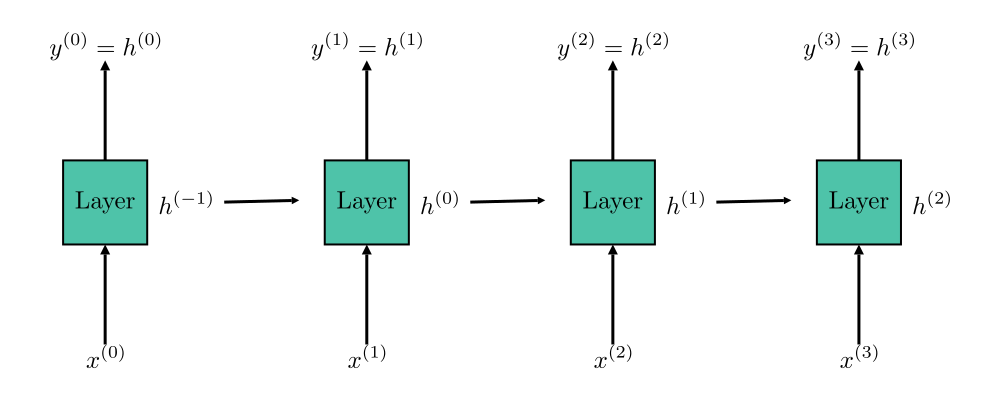
\includegraphics[width=\textwidth]{assets/images/rnn-unfolding.png}
    \caption{Dépliement temporel d'un \glsfmtshort{rnn} sur une entrée de longueur 4.}
    \label{fig.rnn-unfold}
\end{figure}

Chaque état caché \(h^{(i)}\) contient de l'information sur tous les \(x^{(j)},\ j\le i\).
En particulier, \(h^{(n)}\) contient de l'information sur toute la séquence \(x\).
Un encodeur récurrent peut donc retourner son dernier état caché comme vecteur d'encodage~\cite{deep-nmt-survey}.

De sa part, un décodeur récurrent peut conditionner sur l'encodage 
et passer ses états cachés à une couche supplémentaire 
qui les interprète comme plongements des éléments de la sortie \(y\)~\cite{Fathi_2021}.
Un tel décodeur n'a pas besoin d'entrée séquentielle 
(voir~Figure~\ref{fig.rnn-enc-dec} et Algorithme~\ref{lst.rnn-enc-dec}).

\begin{figure}[hbt]
    \begin{center}
        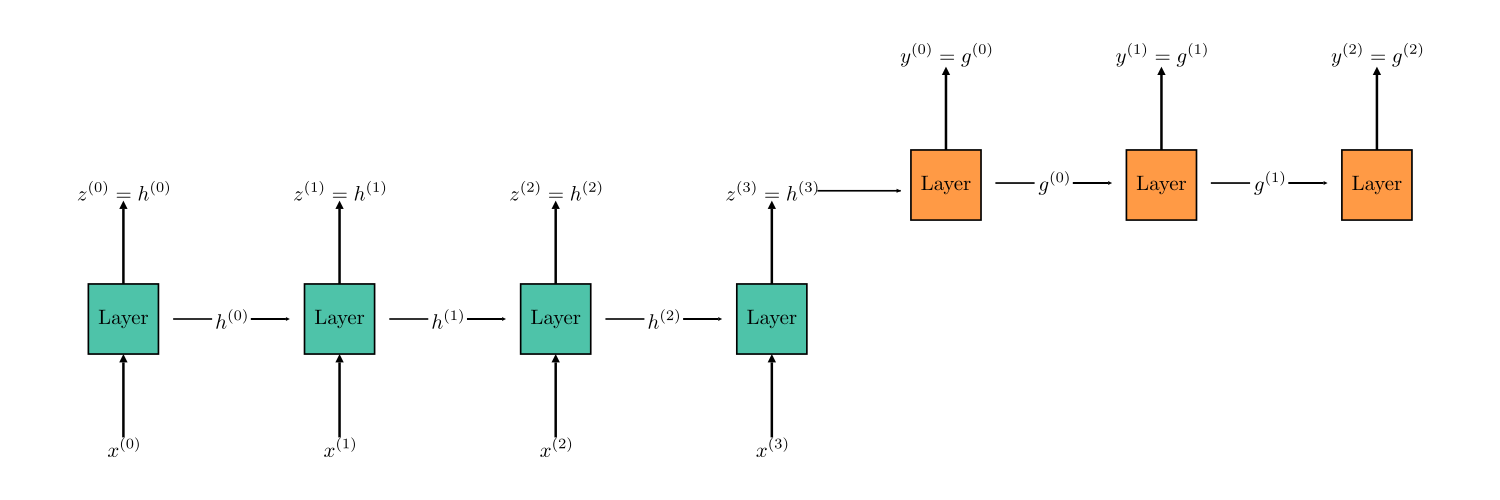
\includegraphics[width=\textwidth]{assets/images/rnn-enc-dec.png}
    \end{center}
    
    \caption[Dépliement temporel d'un encodeur--décodeur récurrent.]
    {Dépliement temporel d'un encodeur--décodeur récurrent  
    sur une entrée de longueur 4 et une sortie de longueur 3.}
    \label{fig.rnn-enc-dec}
\end{figure}

\lstinputlisting[
    language=python, 
    caption={Encodeur--décodeur récurrent.}, 
    label=lst.rnn-enc-dec,
    float=htb,
    firstnumber=1,
    firstline=12,
]
{assets/code/rnn_s2s.py}

\subsubsection{\Glsfmtlong{bptt} et mémoire à court terme}

L'entraînement d'un \gls{rnn} sur un exemple se fait en le dépliant, 
puis en entraînant le \gls{ffn} qui résulte par rétro-propagation.
L'algorithme résultant s'appelle la \gls{bptt}.
Cela est problématique, car la taille de l'entrée n'est théoriquement pas bornée.
Par conséquent, la profondeur effective d'un \gls{rnn} ne l'est pas non plus~\cite{Fathi_2021}.

Or, dans l'entraînement d'un réseau de neurones trop profond,
les modules des gradients peuvent atteindre des valeurs trop grandes ou trop petites.
Il s'agit respectivement des problèmes de ``l'explosion du gradient'' 
et de ``la disparition du gradient''~\cite{Basodi_Ji_Zhang_Pan_2020}
Une conséquence de ce phénomène est que 
les \glspl{rnn} simples ont du mal à traiter les entrées pour lesquelles le dépliement temporel est profond,
(i.e les longues entrées).
Cette incapacité à modéliser les corrélations à long terme est appelée 
``mémoire à court terme''~\cite{Bengio_Simard_Frasconi_1994,Informatik_Bengio_Frasconi_Schmidhuber_2003}.


